\documentclass[12pt]{article} \usepackage{url, graphicx}

% page layout
\setlength{\topmargin}{-0.25in}
\setlength{\textheight}{9.5in}
\setlength{\headheight}{0in}
\setlength{\headsep}{0in}

% problem formatting
\newcommand{\problemname}{Problem}
\newcounter{problem}

% math
\newcommand{\dd}{\mathrm{d}}

% primary units
\newcommand{\rad}{\mathrm{rad}}
\newcommand{\kg}{\mathrm{kg}}
\newcommand{\m}{\mathrm{m}}
\newcommand{\s}{\mathrm{s}}

% secondary units
\renewcommand{\deg}{\mathrm{deg}}
\newcommand{\km}{\mathrm{km}}
\newcommand{\mi}{\mathrm{mi}}
\newcommand{\h}{\mathrm{h}}
\newcommand{\ns}{\mathrm{ns}}
\newcommand{\J}{\mathrm{J}}
\newcommand{\eV}{\mathrm{eV}}
\newcommand{\W}{\mathrm{W}}

% derived units
\newcommand{\mps}{\m\,\s^{-1}}
\newcommand{\mph}{\mi\,\h^{-1}}
\newcommand{\mpss}{\m\,\s^{-2}}

% random stuff
\sloppy\sloppypar\raggedbottom\frenchspacing\thispagestyle{empty}

\begin{document}

\noindent
Name: \rule[-1ex]{0.55\textwidth}{0.1pt}
NetID: \rule[-1ex]{0.2\textwidth}{0.1pt}

\section*{NYU Physics I---Term Exam 6}

\paragraph{\problemname~\theproblem:}\refstepcounter{problem}%
For the elliptical orbit shown, roughly what is the eccentricity?
(From Lecture on 2016-11-16.)\\
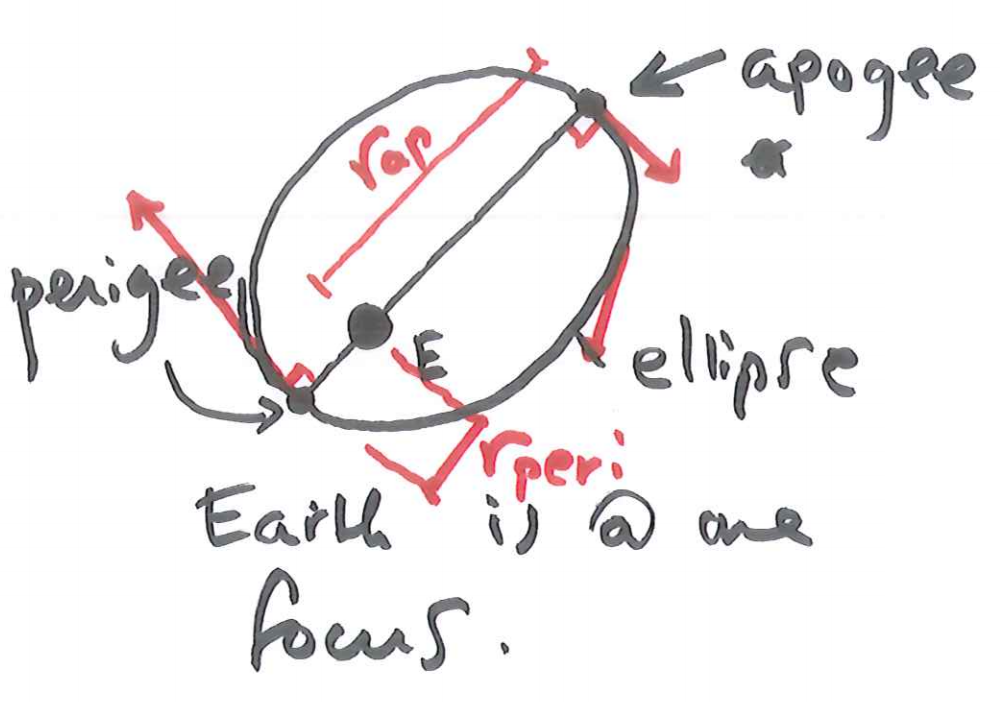
\includegraphics[width=2.5in]{./ellipse.png}

\vfill

\paragraph{\problemname~\theproblem:}\refstepcounter{problem}%
In the twin paradox, which twin ages more? The one on the geodesic, or
the one who changes reference frames? (From Lecture on 2017-12-05.)

\vfill

\paragraph{\problemname~\theproblem:}\refstepcounter{problem}%
What is the speed of a package orbiting on a circular orbit right near
the surface of the Earth? Give your answer in $\mps$. (From Problem Set 11.)

\vfill
~
\clearpage

\paragraph{\problemname~\theproblem:}\refstepcounter{problem}%
Muons have a half-life of $2\times 10^{-8}\,\s$ in their rest
frame. When they are moving at a speed of $0.99\,c$ through the
lab, what would their lab-frame (that is, time-dilated) half-life be?
(From Problem Set 13.)

\vfill

\paragraph{\problemname~\theproblem:}\refstepcounter{problem}%
If the Earth were half as massive as it is, but were still
on a near-circular orbit at its current Earth--Sun distance, how much
longer or shorter would the year be? (From the recitation on orbits.)

\vfill

\paragraph{\problemname~\theproblem:}\refstepcounter{problem}%
What is the spacetime interval between the two events $A$ and $B$?
$$A = (c\,t_A, x_A) = (1\,\m, 4\,\m) $$
$$B = (c\,t_B, x_B) = (8\,\m, 2\,\m) $$
Don't forget your units. (From the recitation on the interval.)

\vfill
~
\end{document}
